\documentclass[aspectratio=169]{beamer}

% because we need to claim weird things
\newtheorem{claim}{Claim}
\newtheorem{defn}{Definition}
%\newtheorem{lemma}{Lemma}
\newtheorem{thm}{Theorem}
\newtheorem{vita}{Vit\ae}
\newtheorem{qotd}{Quote of the Day}

\usepackage{algorithm}
\usepackage{algpseudocode}
\usepackage{listings}
\usepackage{color}
\usepackage{graphics}
\usepackage{ulem}
\bibliographystyle{unsrt}

% background image
\usebackgroundtemplate%
{%
    
\includegraphics[width=\paperwidth,height=\paperheight]{../artifacts/stemulus.pdf}%
}
\setbeamertemplate{caption}[numbered]
\lstset{%
	breaklines=true,
	captionpos=b,
	frame=single,
	keepspaces=true,
	showstringspaces=false
}

% page numbers
\addtobeamertemplate{navigation symbols}{}{%
    \usebeamerfont{footline}%
    \usebeamercolor[fg]{footline}%
    \hspace{1em}%
    \insertframenumber/\inserttotalframenumber
}

% presentation header
\usetheme{Warsaw}
\title{Big Data in a Big World}
\author{Dylan Lane McDonald}
\institute{CNM STEMulus Center\\Web Development with PHP}
\date{\today}

\begin{document}
\lstset{language=Java}
\begin{frame}
\titlepage
\end{frame}

\begin{frame}
\frametitle{Outline}
\tableofcontents
\end{frame}

\section{Big Data in a Big World}
\begin{frame}
\frametitle{Big Data in a Big World}
Data from other sites can be integrated into your site using external APIs.

\mbox{}\\
\begin{defn}
An \textbf{Application Programming Interface (API)} is a publicly available set of functions or methods from an external source.
\end{defn}

\mbox{}\\
All the PHP and JavaScript methods \& functions we've used so far are included as part of the core PHP \& JavaScript API. jQuery is also an API we've used in this class. Another example of an API we've used is \texttt{mysqli}. For the purposes of this discussion, we will be using APIs that allow access to external data.
\end{frame}

\begin{frame}
\frametitle{Acquiring Data from an API}
\begin{figure}
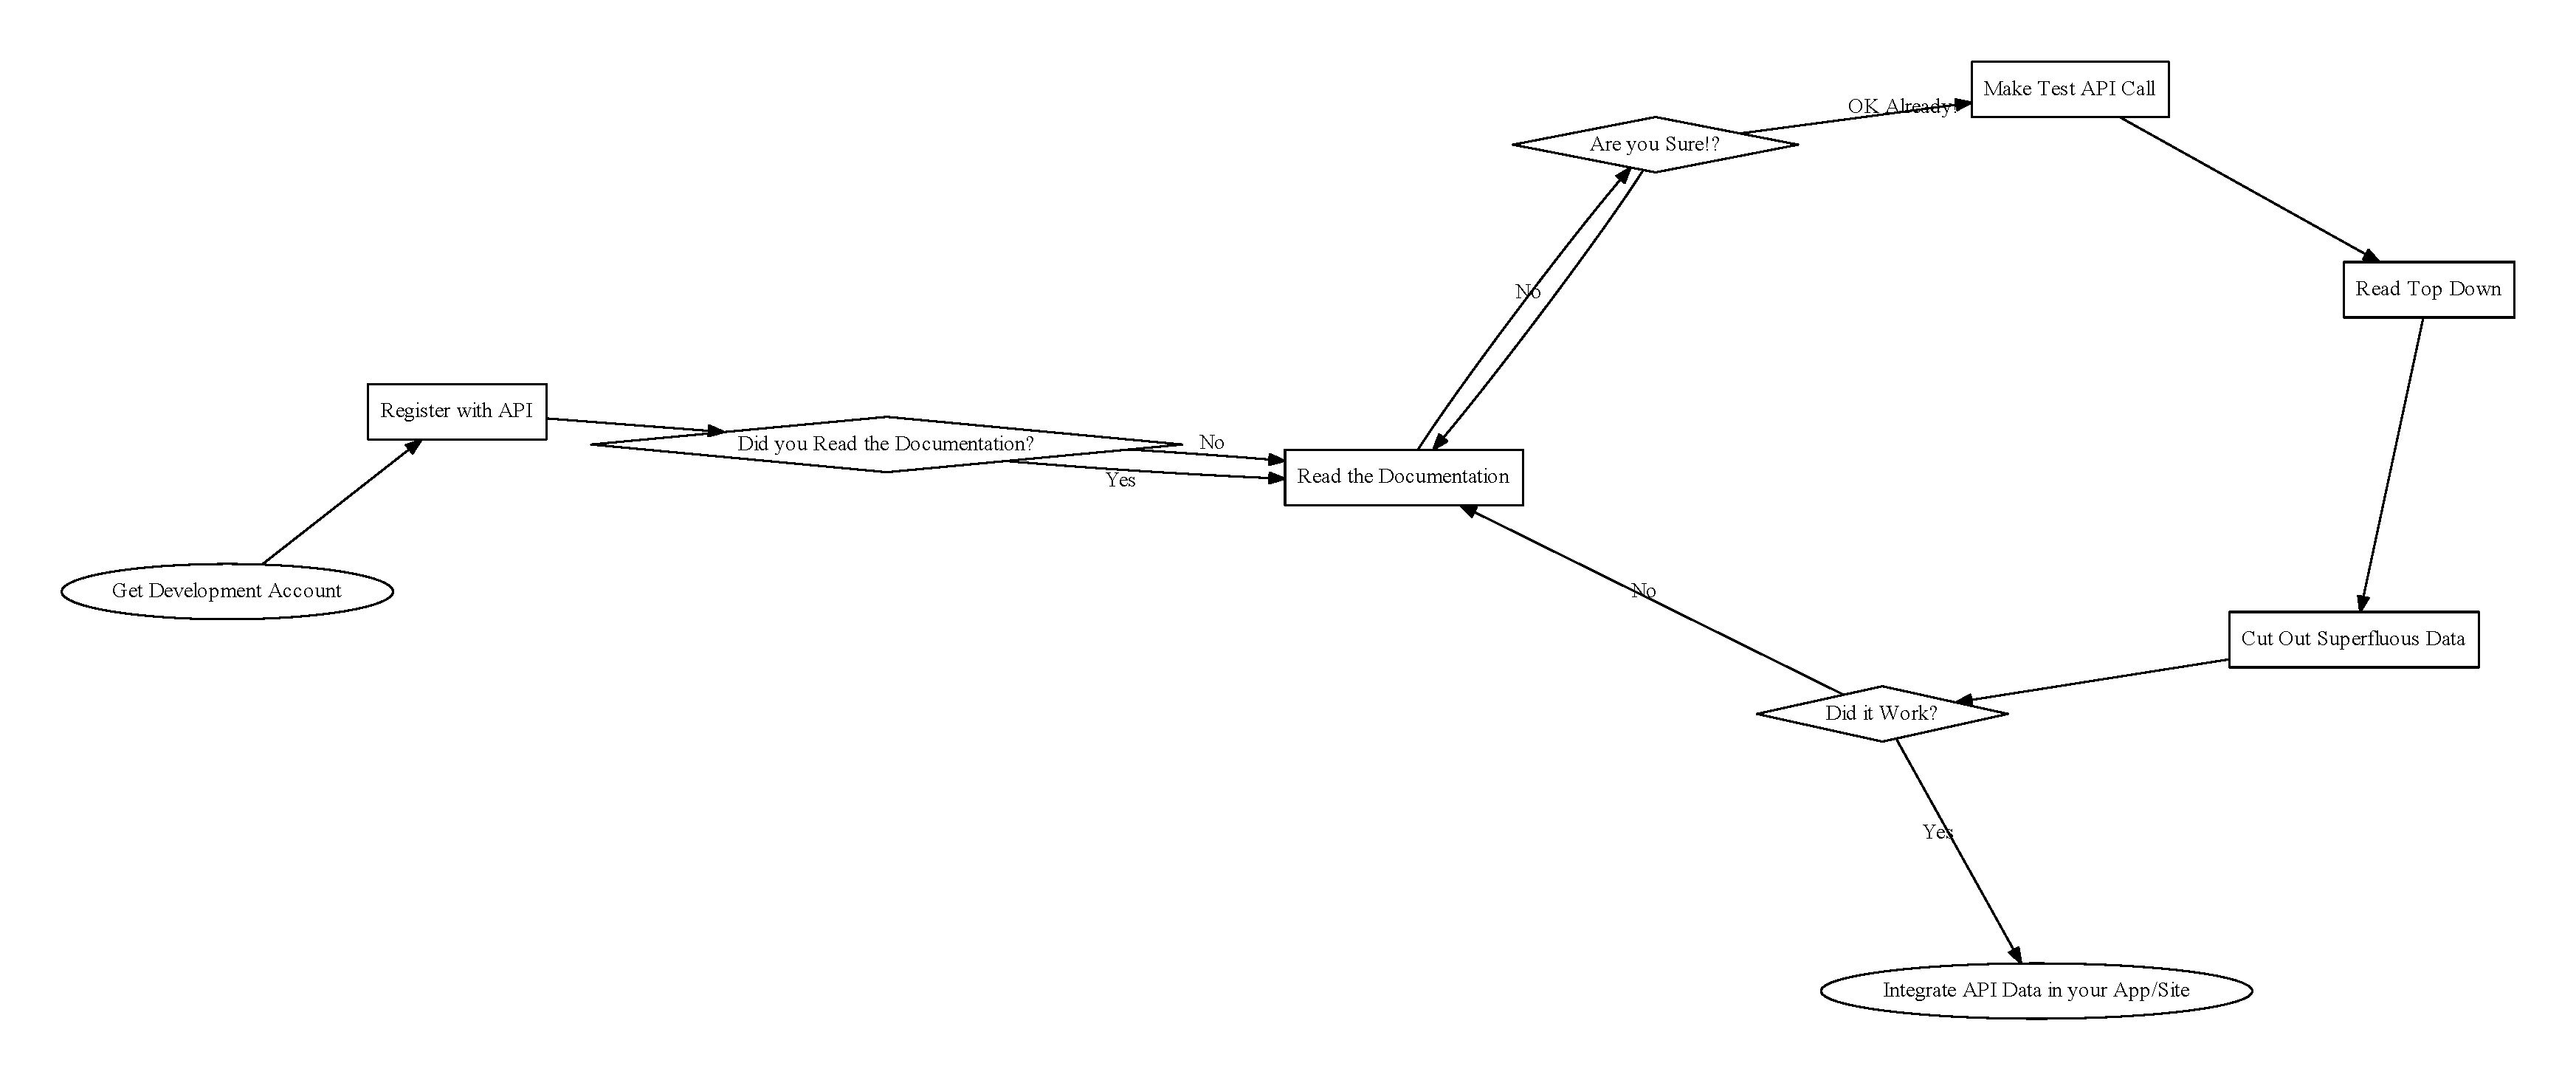
\includegraphics[scale=0.2]{../artifacts/json-roadmap.pdf}
\caption{Acquiring Data from an API}
\label{fig:jsonflow}
\end{figure}
\end{frame}

\section{Data Formats}
\begin{frame}
\frametitle{Data Formats}
The following data formats are available. These are listed in order of preference both in class and in industry.
\begin{enumerate}
	\item \textbf{JSON}: \textbf{J}ava\textbf{S}cript \textbf{O}bject \textbf{N}otation. A simplified, compact notation for representing objects. All major languages have support for writing JSON strings to send to an API, as well as reading JSON strings and converting them to their own internal objects.
	\item \textbf{SOAP}: Used to stand for \textbf{S}imple \textbf{O}bject \textbf{A}ccess \textbf{P}rotocol. SOAP is a modification on XML and standardizes the format of the messages being sent to \& from sites.
	\item \textbf{XML} E\textbf{x}tensible \textbf{M}arkup \textbf{L}anguage. \textbf{XML}: allows one to define one's own markup language and use these tags to house the data being exchanged.
\end{enumerate}
\end{frame}
\end{document}